% chapter1.tex - First chapter

\chapter{Álgebra Lineal}

% Optional: Add a mini table of contents at the beginning of the chapter
\minitoc

% Optional: Add an epigraph/quote at the beginning of the chapter
\epigraph{\textit{La inteligencia es la capacidad de adaptarse al cambio.}}{Albert Einstein}

El álgebra lineal constituye el fundamento matemático de la inteligencia artificial, proporcionando el lenguaje y las
herramientas esenciales para representar y manipular datos, modelos y algoritmos. Este capítulo presenta una revisión
sistemática de conceptos necesarios para el trabajo con \gls{vector}es y \gls{matriz}es. 

\section{Matrices}

\begin{definition}[Matriz]
Una \textbf{\gls{matriz}} de orden $m \times n$ sobre un campo $\mathbb{K}$ es un arreglo rectangular de elementos $a_{ij}
\in \mathbb{K}$ (llamados entradas o coeficientes), donde $i = 1,\ldots,m$ y $j = 1,\ldots,n$, organizados en $m$ filas
y $n$ columnas. Se denota como:
    
\[ A = \begin{bmatrix}
a_{11} & a_{12} & \cdots & a_{1n} \\
a_{21} & a_{22} & \cdots & a_{2n} \\
\vdots & \vdots & \ddots & \vdots \\
a_{m1} & a_{m2} & \cdots & a_{mn}
\end{bmatrix} \]
o de forma abreviada como $A = (a_{ij})_{m\times n}$.
\end{definition}

El conjunto de todas las matrices de orden $m \times n$ con coeficientes en $\mathbb{K}$ se denota por $M_{m
\times n}(\mathbb{K})$. Cuando el número de filas coincide con el número de columnas, se dice que la matriz es
\textbf{\gls{matriz-cuadrada}}. El conjunto de todas las matrices cuadradas de orden $n$ con coeficientes en $\mathbb{K}$ se denota
por $\mathcal{M}_n(\mathbb{K})$, que es equivalente a escribir $\mathcal{M}_{n \times n}(\mathbb{K})$. 

Cada posición en una matriz está identificada por dos índices: uno para la fila y otro para la columna. El elemento que
se encuentra en la intersección de la fila $i$-ésima y la columna $j$-ésima se denomina \textbf{entrada $(i,j)$-ésima}
de la matriz $A$. Por convención, este elemento se denota como $a_{ij}$, lo que permite representar de manera
compacta a la matriz $A$ mediante la notación $(a_{ij})$. 

\begin{definition}[Columna y fila de una matriz]
Sea $A = (a_{ij}) \in \mathcal{M}_{m\times n}(\mathbb{K})$. Dado $j \in \{1,\ldots,n\}$ la matriz
\[
\begin{bmatrix}
a_{1j} \\
\vdots \\
a_{mj}
\end{bmatrix} \in \mathcal{M}_{m\times 1}(\mathbb{K})
\]
se llama \textbf{columna $j$-ésima} de $A$ y se denota como $A_{{c(j)}}$, y dado $i \in \{1,\ldots,m\}$ la matriz
\[
\begin{bmatrix}
a_{i1} & \cdots & a_{in}
\end{bmatrix} \in \mathcal{M}_{1\times n}(\mathbb{K})
\]
se denomina \textbf{fila $i$-ésima} de $A$ y se denota como $A_{{r(i)}}$. 
\end{definition}

A continuación se presentan algunos ejemplos de matrices.

\begin{example}
La \textbf{matriz nula} $0 \in \mathcal{M}_{m\times n}(\mathbb{K})$ es aquella con $m$ filas y $n$ columnas cuyas
entradas son todas iguales a 0. En algunas ocasiones escribiremos $0_{m\times n}$ para denotar a la matriz nula de orden
$m \times n$.
\end{example}

\begin{example}
Se dice que una matriz cuadrada $D = (d_{ij}) \in \mathcal{M}_n(\mathbb{K})$ es \textbf{diagonal} si $d_{ij} = 0$ para
todo $i \neq j$. En otras palabras, una matriz diagonal es aquella que solo tiene elementos no nulos en su diagonal
principal. Utilizaremos la notación
\[
\text{diag}(\lambda_1,\ldots,\lambda_n),
\]
con $\lambda_i \in \mathbb{K}$, $i = 1,\ldots,n$, para denotar la matriz diagonal $D$ donde $d_{ii} = \lambda_i$ para $i
= 1,\ldots,n$. Es decir, 
\[
D = \text{diag}(\lambda_1,\ldots,\lambda_n) = \begin{bmatrix}
\lambda_1 & 0 & \cdots & 0 \\
0 & \lambda_2 & \cdots & 0 \\
\vdots & \vdots & \ddots & \vdots \\
0 & 0 & \cdots & \lambda_n
\end{bmatrix}
\]
\end{example}

\begin{example}
La \textbf{matriz identidad} $I_n \in \mathcal{M}_n(\mathbb{K})$ es aquella con $n$ filas y $n$ columnas cuyas
entradas son todas iguales a 0 excepto las de la diagonal principal, que son iguales a 1. Es decir,
\[
I_n = 
\begin{bmatrix}
1 & 0 & \ldots & 0 \\
0 & 1 & \ldots & 0 \\
\vdots & \vdots & \ddots & \vdots \\
0 & 0 & \ldots & 1
\end{bmatrix}.
\]

Con la notación habitual de la \textit{delta de Kronecker}
\[
\delta_{ij} = 
\begin{cases}
1 & \text{si } i = j \\
0 & \text{si } i \neq j
\end{cases}
\]
se tiene que $I_n = (\delta_{ij}) \in \mathcal{M}_n(\mathbb{K})$.
\end{example}

\begin{definition}[Igualdad de matrices]
Dos matrices $A=(a_{ij})$ y $B=(b_{ij})$ en $\mathcal{M}_{m\times n}(\mathbb{K})$ son \textbf{iguales} si y solo si
tienen el mismo orden y sus entradas correspondientes son iguales; es decir: 
\[
A = B \iff a_{ij} = b_{ij} \text{ para todo } i = 1,\ldots,m \text{ y } j = 1,\ldots,n
\]
\end{definition}

\begin{definition}[Submatriz]
Sea $A \in \mathcal{M}_{m\times n}(\mathbb{K})$. Llamaremos \textbf{submatriz} de $A$ a cualquier
matriz obtenida a partir de $A$ suprimiendo algunas de sus filas y/o columnas. Si $I \subseteq \{1,\ldots,m\}$ y $J
\subseteq \{1,\ldots,n\}$ son subconjuntos de índices, denotaremos por $A_{IJ}$ a la submatriz formada por las filas
indexadas por $I$ y las columnas indexadas por $J$. 
\end{definition}

\begin{example}
Consideremos la matriz $A \in \mathcal{M}_{5\times 5}(\mathbb{K})$ dada por:
\[
A = \begin{bmatrix}
1 & 2 & 3 & 4 & 5 \\
6 & 7 & 8 & 9 & 10 \\
11 & 12 & 13 & 14 & 15 \\
16 & 17 & 18 & 19 & 20 \\
21 & 22 & 23 & 24 & 25
\end{bmatrix}.
\]
Si tomamos los subconjuntos de índices $I = \{1,3,4\}$ y $J = \{2,4,5\}$, entonces la submatriz $A_{IJ}$ es:
\[
A_{IJ} = \begin{bmatrix}
2 & 4 & 5 \\
12 & 14 & 15 \\
17 & 19 & 20
\end{bmatrix}
\]
que corresponde al conjunto de subindices $I \times J$ de la matriz $A$.

Para visualizar mejor este proceso de selección de submatriz, consideremos el siguiente diagrama:

% Diagrama de submatriz alineado verticalmente
\begin{center}
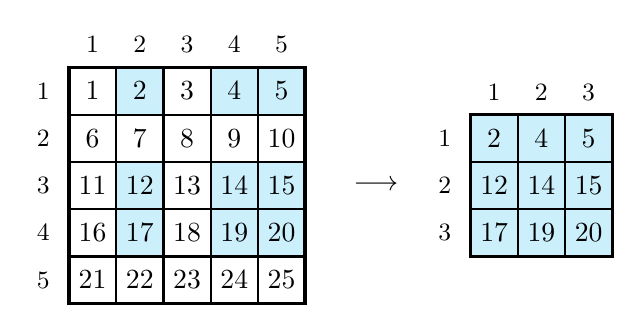
\begin{tikzpicture}[every node/.style={font=\normalsize}, scale=0.6, baseline=(current bounding box.center)]

% Matriz original (5x5)
\begin{scope}[yshift=0cm]
% Relleno de submatriz seleccionada (filas 1,3,4 y columnas 2,4,5)
\foreach \i/\y in {1/4,3/2,4/1} {
\foreach \j/\x in {2/1,4/3,5/4} {
    \fill[cyan!20] (\x,\y) rectangle (\x+1,\y+1);
}
}

% Cuadrícula principal
\draw[very thick, black] (0,0) rectangle (5,5);
\foreach \x in {1,...,4}
\draw[thick, black] (0,\x) -- (5,\x);
\foreach \x in {1,...,4}
\draw[thick, black] (\x,0) -- (\x,5);

% Números en la matriz
\node at (0.5,4.5) {1}; \node at (1.5,4.5) {2}; \node at (2.5,4.5) {3}; \node at (3.5,4.5) {4}; \node at (4.5,4.5) {5};
\node at (0.5,3.5) {6}; \node at (1.5,3.5) {7}; \node at (2.5,3.5) {8}; \node at (3.5,3.5) {9}; \node at (4.5,3.5) {10};
\node at (0.5,2.5) {11}; \node at (1.5,2.5) {12}; \node at (2.5,2.5) {13}; \node at (3.5,2.5) {14}; \node at (4.5,2.5) {15};
\node at (0.5,1.5) {16}; \node at (1.5,1.5) {17}; \node at (2.5,1.5) {18}; \node at (3.5,1.5) {19}; \node at (4.5,1.5) {20};
\node at (0.5,0.5) {21}; \node at (1.5,0.5) {22}; \node at (2.5,0.5) {23}; \node at (3.5,0.5) {24}; \node at (4.5,0.5) {25};

% Etiquetas de filas (izquierda)
\foreach \i in {1,...,5} {
\node[left, font=\small, text=black] at (-0.2,5.5-\i) {\i};
}
% Etiquetas de columnas (arriba)
\foreach \j in {1,...,5} {
\node[above, font=\small, text=black] at (\j-0.5,5.1) {\j};
}
\end{scope}

% Flecha elegante, centrada verticalmente respecto a la matriz
\node (flecha) at (6.5,2.5) {\normalsize$\longrightarrow$};

% Submatriz resultante (3x3), centrada verticalmente respecto a la matriz original
\begin{scope}[xshift=8.5cm, yshift=1cm]
% Relleno
\fill[cyan!20] (0,0) rectangle (3,3);
% Cuadrícula
\draw[very thick, black] (0,0) rectangle (3,3);
\foreach \x in {1,2}
\draw[thick, black] (0,\x) -- (3,\x);
\foreach \x in {1,2}
\draw[thick, black] (\x,0) -- (\x,3);
% Números en la submatriz
\node at (0.5,2.5) {2}; \node at (1.5,2.5) {4}; \node at (2.5,2.5) {5};
\node at (0.5,1.5) {12}; \node at (1.5,1.5) {14}; \node at (2.5,1.5) {15};
\node at (0.5,0.5) {17}; \node at (1.5,0.5) {19}; \node at (2.5,0.5) {20};
% Etiquetas de filas y columnas
\foreach \i in {1,...,3} {
\node[left, font=\small, text=black] at (-0.2,3.5-\i) {\i};
\node[above, font=\small, text=black] at (\i-0.5,3.1) {\i};
}
\end{scope}

\end{tikzpicture}
\end{center}

donde las casillas sombreadas corresponden a los elementos seleccionados para formar la submatriz $A_{IJ}$ con $I =
\{1,3,4\}$ y $J = \{2,4,5\}$. 
\end{example}

\section{Operaciones con matrices}

\begin{definition}[Suma de matrices]
La suma de dos matrices $A \in \mathcal{M}_{m\times n}(\mathbb{K})$, $B \in \mathcal{M}_{m\times n}(\mathbb{K})$ se
define como la suma elemento a elemento, es decir, 
\[
A + B := 
\begin{bmatrix} 
a_{11} + b_{11} & \cdots & a_{1n} + b_{1n} \\
\vdots & & \vdots \\
a_{m1} + b_{m1} & \cdots & a_{mn} + b_{mn}
\end{bmatrix}
\in \mathcal{M}_{m\times n}(\mathbb{K}).
\]
\end{definition}

La suma de matrices cumple las siguientes propiedades fundamentales:

\begin{enumerate}
\item \textbf{Asociatividad:} Para cualesquiera matrices $A$, $B$, $C \in \mathcal{M}_{m \times n}(k)$, se cumple que
$(A + B) + C = A + (B + C)$. 

\item \textbf{Conmutatividad:} Para cualesquiera matrices $A$, $B \in \mathcal{M}_{m \times n}(k)$, se cumple que $A + B
= B + A$. 

\item \textbf{Elemento neutro:} La matriz nula $0 \in \mathcal{M}_{m \times n}(k)$ actúa como elemento neutro de la
suma, es decir, para toda matriz $A \in \mathcal{M}_{m \times n}(k)$ se cumple que $A + 0 = 0 + A = A$.

\item \textbf{Elemento opuesto:} Para toda matriz $A = (a_{ij}) \in \mathcal{M}_{m \times n}(k)$, existe una matriz
opuesta $-A = (-a_{ij})$ tal que $A + (-A) = (-A) + A = 0$. Esta matriz opuesta se obtiene multiplicando cada elemento
de $A$ por $-1$.
\end{enumerate}

Estas propiedades dotan al conjunto $\mathcal{M}_{m \times n}(k)$ de una estructura de grupo abeliano respecto a la
operación suma.

\begin{definition}[Producto de un escalar por una matriz]
Sea $A = (a_{ij}) \in \mathcal{M}_{m \times n}(k)$ y $\lambda \in k$. Se define el producto de $\lambda$ por $A$ como la
matriz 
\[
\lambda \cdot A := 
\begin{bmatrix}
\lambda a_{11} & \cdots & \lambda a_{1n} \\
\vdots & \ddots & \vdots \\
\lambda a_{m1} & \cdots & \lambda a_{mn}
\end{bmatrix}
\in \mathcal{M}_{m \times n}(k),
\]
esto es, el producto de un escalar por una matriz es la matriz que resulta al multiplicar cada una de las entradas de la
matriz por el escalar. 
\end{definition}

Para $\lambda, \mu \in \mathbb{K}$ y $A, B \in \mathcal{M}_{m \times n}(\mathbb{K})$, el producto de un escalar por una
matriz cumple las siguientes propiedades:
\begin{enumerate}
\item \textbf{Distributividad respecto a la suma de escalares:} $\lambda(A + B) = \lambda A + \lambda B$.
\item \textbf{Distributividad respecto a la suma de matrices:} $(\lambda + \mu)A = \lambda A + \mu A$.
\item \textbf{Compatibilidad con la multiplicación de escalares:} $(\lambda \mu)A = \lambda(\mu A)$.
\item \textbf{Asociatividad del producto por escalares:} $\lambda(\mu A) = (\lambda \mu)A$.
\end{enumerate}


\begin{definition}[Producto de matrices]
Sean $A = (a_{ij}) \in \mathcal{M}_{m\times p}(\mathbb{K})$ y $B = (b_{ij}) \in \mathcal{M}_{p\times n}(\mathbb{K})$ dos
matrices. El producto $C = AB = (c_{ij}) \in \mathcal{M}_{m\times n}(\mathbb{K})$  es una matriz cuyos elementos
$c_{ij}$ se calculan como: 
\begin{equation}
c_{ij} = \sum_{l=1}^{p} a_{il}b_{lj}, \quad i = 1,\ldots,m, \quad j = 1,\ldots,n.
\tag{2.13}
\end{equation}
\end{definition}

Para visualizar mejor cómo se realiza este producto, consideremos la siguiente representación gráfica:

% Producto de matrices: representación gráfica (tamaño ajustado)
\begin{center}
\begin{tikzpicture}[
every node/.style={font=\normalsize},
scale=0.5,
mat/.style={matrix of math nodes, left delimiter={[}, right delimiter={]}, nodes={text width=1em, text height=1em, align=center}
},
node distance=0.15cm and 0.15cm
]
\pgfdeclarelayer{background}
\pgfsetlayers{background,main}

% Matriz A
\matrix (A) [mat] at (0,0) {
a_{11} & a_{12} & \cdots & a_{1p} \\
\vdots & \vdots & \ddots & \vdots \\
a_{i1} & a_{i2} & \cdots & a_{ip} \\
\vdots & \vdots & \ddots & \vdots \\
a_{m1} & a_{m2} & \cdots & a_{mp} \\
};
\begin{pgfonlayer}{background}
\fill[green!20,rounded corners]
([xshift=-1.5pt,yshift=1.5pt]A-3-1.north west) rectangle
([xshift=1.5pt,yshift=-1.5pt]A-3-4.south east);
\end{pgfonlayer}

% Signo de multiplicación, perfectamente centrado
\node (times) [right=of A] {\large $\times$};

% Matriz B, alineada con la fila resaltada de A
\matrix (B) [mat, right=of times] {
b_{11} & \cdots & b_{1j} & \cdots & b_{1n} \\
b_{21} & \cdots & b_{2j} & \cdots & b_{2n} \\
\vdots & \ddots & \vdots & \ddots & \vdots \\
b_{p1} & \cdots & b_{pj} & \cdots & b_{pn} \\
};
\begin{pgfonlayer}{background}
\fill[green!20,rounded corners]
([xshift=-1.5pt,yshift=1.5pt]B-1-3.north west) rectangle
([xshift=1.5pt,yshift=-1.5pt]B-4-3.south east);
\end{pgfonlayer}

% Signo de igual, perfectamente centrado
\node (equals) [right=of B] {\large $=$};

% Matriz C, alineada con la fila resaltada de A y la columna de B
\matrix (C) [mat, right=of equals] {
c_{11} & \cdots & c_{1j} & \cdots & c_{1n} \\
\vdots & \ddots & \vdots & \ddots & \vdots \\
c_{i1} & \cdots & c_{ij} & \cdots & c_{in} \\
\vdots & \ddots & \vdots & \ddots & \vdots \\
c_{m1} & \cdots & c_{mj} & \cdots & c_{mn} \\
};
\begin{pgfonlayer}{background}
\fill[blue!20,rounded corners]
([xshift=-1.5pt,yshift=1.5pt]C-3-3.north west) rectangle
([xshift=1.5pt,yshift=-1.5pt]C-3-3.south east);
\end{pgfonlayer}

% Añadir flechas curvas para mostrar la multiplicación
\draw[->,green!50!black,thick,opacity=0.3] (A-3-1.east) .. controls +(1,0.5) .. (B-1-3.west);
\draw[->,green!50!black,thick,opacity=0.3] (A-3-2.east) .. controls +(1,0.3) .. (B-2-3.west);
\draw[->,green!50!black,thick,opacity=0.3] (A-3-4.east) .. controls +(1,-0.3) .. (B-4-3.west);
\end{tikzpicture}
\end{center}

En el diagrama anterior, se muestra cómo cada elemento $c_{ij}$ del producto (resaltado en azul) se obtiene del producto
escalar entre la fila $i$-ésima de $A$ (resaltada  en verde) y la columna $j$-ésima de $B$ (resaltada en verde). 
Utilizamos la notación $A_{r(i)}$ para referirnos a la fila $i$-ésima de $A$ y $B_{c(j)}$ para la columna $j$-ésima de
$B$.

\begin{remark}
Las matrices solo pueden multiplicarse si sus dimensiones «vecinas» coinciden. Por ejemplo, una matriz $A$ de
dimensión $n \times p$ puede multiplicarse con una matriz $B$ de dimensión $p \times m$, pero solo por la izquierda: 
\[
\underset{n \times p}{A} \cdot \underset{p \times m}{B} = \underset{n \times m}{C}
\]
El producto $BA$ no está definido si $m \neq n$ ya que las dimensiones vecinas no coinciden.
\end{remark}

\begin{remark}
La multiplicación de matrices \textit{no} está definida como una operación elemento a elemento, es decir, $c_{ij} \neq
a_{ij}b_{ij}$ (incluso si el tamaño de $A$ y $B$ fuera apropiado). Este tipo de multiplicación elemento a elemento
aparece frecuentemente en lenguajes de programación cuando multiplicamos arreglos (multidimensionales) entre sí, y se
denomina \textit{producto de Hadamard}.
\end{remark}

Ahora que hemos definido la multiplicación de matrices, la suma de matrices y la matriz identidad, veamos algunas
propiedades de las operaciones matriciales:
\begin{enumerate}
\item \textbf{Propiedad asociativa de la multiplicación:} Sea $A \in \mathcal{M}_{m \times n}$, $B \in \mathcal{M}_{n
\times p}$, $C \in \mathcal{M}_{p \times q}$, entonces 
\[(AB)C = A(BC)\]
Esta propiedad nos permite calcular productos de tres o más matrices en cualquier orden de agrupación.

\item \textbf{Propiedades distributivas:} Sea $A, B \in \mathcal{M}_{m \times n}$, $C, D \in \mathcal{M}_{n \times p}$,
entonces 
\[(A + B)C = AC + BC\]
\[A(C + D) = AC + AD\]
La multiplicación matricial distribuye tanto por la izquierda como por la derecha respecto a la suma.

\item \textbf{Propiedades de la matriz identidad:} Sea $A \in \mathcal{M}_{m \times n}$, entonces
\[I_mA = AI_n = A\]
La matriz identidad actúa como elemento neutro de la multiplicación. Es importante observar que $I_m \neq I_n$ cuando $m 
\neq n$, y que necesitamos matrices identidad de diferentes dimensiones para multiplicar por la izquierda ($I_m$) y por
la derecha ($I_n$).
\end{enumerate}

Con las propiedades anteriores, el conjunto $\mathcal{M}_{m \times n}(\mathbb{K})$ con las operaciones de suma y
producto por escalares, y con la matriz identidad, cumple las propiedades de un anillo conmutativo con unidad.

\begin{definition}[Matriz traspuesta]
Dada una matriz $A \in \mathcal{M}_{m \times n}(\mathbb{K})$, definimos su \textbf{\gls{matriz-transpuesta}} $A^\top \in
\mathcal{M}_{n \times m}(\mathbb{K})$ como aquella que se obtiene al intercambiar filas por columnas, es decir, $
(A^\top)_{ij} = A_{ji}$.
\end{definition}

\begin{example}
Si tenemos la matriz
\[
A = \begin{pmatrix}
1 & 2 & 3 \\
4 & 5 & 6
\end{pmatrix} \in \mathcal{M}_{2 \times 3}(\mathbb{R})
\]
su matriz traspuesta es
\[
A^\top = \begin{pmatrix}
1 & 4 \\
2 & 5 \\
3 & 6
\end{pmatrix} \in \mathcal{M}_{3 \times 2}(\mathbb{R})
\]
Observe que las columnas de $A^\top$ son las filas de $A$ y viceversa.
\end{example}

\begin{definition}[Matriz simétrica y antisimétrica]
Una matriz cuadrada $A = (a_{ij}) \in \mathcal{M}_n(\mathbb{K})$ es:
\begin{enumerate}
\item \textbf{Simétrica} si $A = A^\top$, es decir, si $a_{ij} = a_{ji}$ para todo $i,j$.
\item \textbf{Antisimétrica} si $A = -A^\top$, es decir, si $a_{ij} = -a_{ji}$ para todo $i,j$.
\end{enumerate}
\end{definition}

\begin{example}
Consideremos las siguientes matrices:
\[
B = \begin{pmatrix}
1 & 2 \\
2 & 3
\end{pmatrix} \quad \text{y} \quad
C = \begin{pmatrix}
0 & 1 \\
-1 & 0
\end{pmatrix}
\]
La matriz $B$ es \gls{matriz-simetrica} ya que $B = B^\top$, mientras que $C$ es \gls{matriz-antisimetrica} pues $C = -C^\top$. Puede verificarse
esto observando que en $B$, los elementos simétricos respecto a la diagonal principal son iguales ($b_{12} = b_ {21} =
2$), mientras que en $C$, los elementos simétricos son opuestos ($c_{12} = -c_{21} = 1$).
\end{example}
    
\begin{definition}[Matriz invertible]
Una matriz $A \in \mathcal{M}_n(\mathbb{K})$ es \textbf{invertible} (o \textbf{no singular}) si existe una matriz $B \in
\mathcal{M}_n(\mathbb{K})$ tal que $AB = BA = I_n$. En tal caso, la matriz $B$ es única y se denomina \textbf{\gls{matriz-inversa} de $A$}, denotándose por $A^{-1}$.
\end{definition}

\begin{example}
Consideremos la matriz
\[
A = \begin{pmatrix}
0 & 1 \\
1 & 0
\end{pmatrix}
\]
Su matriz inversa es
\[
A^{-1} = \begin{pmatrix}
0 & 1 \\
1 & 0
\end{pmatrix}
\]
En efecto, podemos verificar que $AA^{-1} = A^{-1}A = I_2$ realizando el producto:
\[
AA^{-1} = \begin{pmatrix}
0 & 1 \\
1 & 0
\end{pmatrix}
\begin{pmatrix}
0 & 1 \\
1 & 0
\end{pmatrix} =
\begin{pmatrix}
1 & 0 \\
0 & 1
\end{pmatrix} = I_2
\]
En este caso particular, $A$ es su propia inversa, es decir, $A^{-1} = A$. Las matrices con esta propiedad se denominan
\textbf{involutivas}. 
\end{example}


Más adelante daremos un criterio para saber si una matriz es invertible y, en este caso, una fórmula para calcular la
matriz inversa. 

\begin{definition}[Matriz ortogonal]
Una matriz $A \in \mathcal{M}_n(\mathbb{R})$ es \textbf{ortogonal} si su transpuesta coincide con su inversa, es decir,
si $A^\top = A^{-1}$. De forma equivalente, $A$ es ortogonal si y solo si $AA^\top = A^\top A = I_n$. 
\end{definition}

\begin{example}
Consideremos la matriz
\[
A = \begin{pmatrix}
\frac{1}{\sqrt{2}} & \frac{1}{\sqrt{2}} \\
\frac{1}{\sqrt{2}} & -\frac{1}{\sqrt{2}}
\end{pmatrix}
\]
Podemos verificar que $A$ es ortogonal realizando el producto:
\[
A^\top A = \begin{pmatrix}
\frac{1}{\sqrt{2}} & \frac{1}{\sqrt{2}} \\
\frac{1}{\sqrt{2}} & -\frac{1}{\sqrt{2}}
\end{pmatrix}
\begin{pmatrix}
\frac{1}{\sqrt{2}} & \frac{1}{\sqrt{2}} \\
\frac{1}{\sqrt{2}} & -\frac{1}{\sqrt{2}}
\end{pmatrix} =
\begin{pmatrix}
1 & 0 \\
0 & 1
\end{pmatrix} = I_2
\]
Por lo tanto, $A$ es ortogonal.
\end{example}


\begin{definition}[Matriz traspuesta conjugada]
Sea $A = (a_{ij}) \in \mathcal{M}_{m \times n}(\mathbb{C})$. La matriz $A^* = (\overline{a_{ji}}) \in \mathcal{M}_{n
\times m}(\mathbb{C})$  se denomina \textbf{matriz traspuesta conjugada} o \textbf{matriz adjunta}, siendo
$\overline{a_{ji}}$ el  conjugado complejo de $a_{ji}$, para $i = 1, \ldots, m$ y $j = 1, \ldots, n$. Esta operación
combina la transposición de la matriz con la conjugación compleja de sus elementos.
\end{definition}

La matriz traspuesta conjugada tiene varias propiedades importantes:
\begin{enumerate}
\item $(A^*)^* = A$ (involución)
\item Para matrices reales, $A^* = A^\top$, ya que los números reales son iguales a sus conjugados
\item $(AB)^* = B^*A^*$ para matrices compatibles
\item Para escalares $\lambda \in \mathbb{C}$, $(\lambda A)^* = \overline{\lambda}A^*$
\end{enumerate}

Para un vector columna
\[
\mathbf{v} = \begin{pmatrix}
v_1 \\
\vdots \\
v_n
\end{pmatrix} \in \mathbb{C}^n,
\]
su traspuesta conjugada es el vector fila $\mathbf{v}^* = (\overline{v_1}, \ldots, \overline{v_n})$.

\begin{definition}[Matrices especiales complejas]
Sea $A = (a_{ij}) \in \mathcal{M}_n(\mathbb{C})$. Se dice que $A$ es:
\begin{enumerate}
\item \textbf{Hermítica} (o auto-adjunta) si $A = A^*$, es decir, $a_{ij} = \overline{a_{ji}}$ para todo $i, j = 1, 2,
\ldots, n$. Los elementos de la diagonal principal de una matriz hermítica son  necesariamente números reales.

\item \textbf{Unitaria} si $A^* = A^{-1}$, es decir, $AA^* = A^*A = I_n$. Las matrices unitarias son la generalización
compleja de las matrices ortogonales reales. 

\item \textbf{Normal} si $AA^* = A^*A$, es decir, si la matriz conmuta con su traspuesta conjugada.
\end{enumerate}
\end{definition}

\begin{theorem}
Las matrices hermíticas y unitarias tienen propiedades especiales que las relacionan con las matrices normales. En particular:
\begin{enumerate}
\item Toda matriz hermítica o unitaria es también normal.
\item Si $A$ es hermítica, entonces $A=A^*$. Por consiguiente, $AA^* = A A = A^*A$.
\item Si $A$ es unitaria, entonces $AA^*=I_n$ y $A^*A=I_n$. Por consiguiente, $AA^* = A^*A$.
\end{enumerate}
\end{theorem}

\subsection{La traza y el determinante de una matriz}
\begin{definition}[Traza de una matriz]
Sea $A = (a_{ij}) \in \mathcal{M}_n(\mathbb{K})$ una matriz cuadrada de orden $n$. La \textbf{traza} de $A$, denotada
por $\text{tr}(A)$, es la suma de los elementos de su diagonal principal:
\[
\text{tr}(A) = \sum_{i=1}^{n} a_{ii} = a_{11} + a_{22} + \cdots + a_{nn}.
\]
\end{definition}
\begin{example}
Si tenemos la matriz
\[
A = \begin{pmatrix}
1 & 2 & 3 \\
4 & 5 & 6 \\
7 & 8 & 9
\end{pmatrix}
\]
su traza es
\[
\text{tr}(A) = 1 + 5 + 9 = 15.
\]
\end{example}
\begin{definition}[Determinante de una matriz]
Sea $A = (a_{ij}) \in \mathcal{M}_n(\mathbb{K})$ una matriz cuadrada de orden $n$. El \textbf{determinante} de $A$,
denotado por $\det(A)$ o $|A|$, es un escalar que se define por la expresión:
\[
|A| = \sum_{\sigma \in S_n} \mathrm{sign}(\sigma) a_{1\sigma(1)} a_{2\sigma(2)} \cdots a_{n\sigma(n)},
\]
donde $S_n$ es el conjunto de todas las permutaciones de los índices $\{1, 2, \ldots, n\}$ y $\mathrm{sign}(\sigma)$ es
la función signo que asigna $+1$ a las permutaciones pares y $-1$ a las impares. Esta definición se puede expresar de manera
compacta como:
\[
|A| = \sum_{\sigma \in S_n} \mathrm{sign}(\sigma) \prod_{i=1}^{n} a_{i\sigma(i)}.
\]
\end{definition}
Veamos algunos ejemplos de determinantes:
\begin{example}
Consideremos la matriz $A = (a_{ij}) \in \mathcal{M}_2(\mathbb{K})$, entonces su determinante se calcula como:
\[
|A| = a_{11}a_{22} - a_{12}a_{21}.
\]
En donde $S_2 = \{(1,2), (2,1)\}$ y $\mathrm{sign}((1,2)) = 1$, $\mathrm{sign}((2,1)) = -1$. 
\end{example}
\begin{example}
Consideremos la matriz $B = (b_{ij}) \in \mathcal{M}_3(\mathbb{K})$, entonces su determinante se calcula como:
\[
|B| = b_{11}b_{22}b_{33} + b_{12}b_{23}b_{31} + b_{13}b_{21}b_{32} - b_{13}b_{22}b_{31} - b_{12}b_{21}b_{33}
- b_{11}b_{23}b_{32}.
\]
En donde $S_3 = \{(1,2,3), (1,3,2), (2,1,3), (2,3,1), (3,1,2), (3,2,1)\}$ y las funciones signo
son $\mathrm{sign}((1,2,3)) = 1$, $\mathrm{sign}((1,3,2)) = -1$, $\mathrm{sign}((2,1,3)) = -1$, $\mathrm{sign}((2,3,1))
= 1$,  $\mathrm{sign}((3,1,2)) = 1$, y $\mathrm{sign}((3,2,1)) = -1$.
\end{example}

\begin{definition}[Matrices menores]
Sea $A \in \mathcal{M}_{m \times n}(k)$. Para un entero positivo $p$ tal que $p \leq \min(m, n)$, se denomina
\emph{menor de orden $p$}  de $A$ a cualquier determinante de una submatriz cuadrada de $A$ de tamaño $p \times p$.

En el caso en que $A$ es cuadrada ($m = n$), el \textbf{menor principal de orden $p$} es el determinante de la submatriz
obtenida al conservar las primeras $p$ filas y columnas de $A$ (es decir, eliminando las últimas $n - p$ filas y
columnas).
\end{definition}

\begin{definition}[Matriz de cofactores]
Sea $A \in \mathcal{M}_{n \times n}(k)$. La \textbf{matriz de cofactores} de $A$, denotada por $C = (c_{ij})$, es la
matriz  obtenida al calcular el cofactor $c_{ij}$ de cada elemento $a_{ij}$ de $A$. El cofactor se define como:
\[
c_{ij} = (-1)^{i+j} |A_{ij}|,
\]
donde $|A_{ij}|$ es el determinante del menor obtenido al eliminar la fila $i$ y la columna $j$ de $A$.
\end{definition}

\begin{theorem}
Sea $A \in \mathcal{M}_{n \times n}(k)$ una matriz cuadrada de orden $n$. Entonces el determinante de $A$ es igual a la suma de los productos de los elementos de cualquier fila (o columna) de $A$ por
sus cofactores correspondientes, es decir, si elegimos la fila $i$, entonces:
\[
|A| = \sum_{j=1}^{n} a_{ij} c_{ij} = a_{i1}c_{i1} + a_{i2}c_{i2} + \cdots + a_{in}c_{in}.
\]
o si elegimos la columna $j$, entonces:
\[
|A| = \sum_{i=1}^{n} a_{ij} c_{ij} = a_{1j}c_{1j} + a_{2j}c_{2j} + \cdots + a_{nj}c_{nj}.
\]
\end{theorem}

\begin{remark}
Es imporante resaltar que el determinante de la suma de matrices no es igual a la suma de los determinantes, es decir,
en general $|A + B| \neq |A| + |B|$ para matrices $A, B \in \mathcal{M}_{n \times n}(k)$, y por lo tanto, tampoco se $|\lambda A| = \lambda |A|$ para un escalar $\lambda \in k$ y una matriz $A \in \mathcal{M}_{n \times n}(k)$.
\end{remark}

\subsection{Matriz inversa}

